\begin{intersong}
    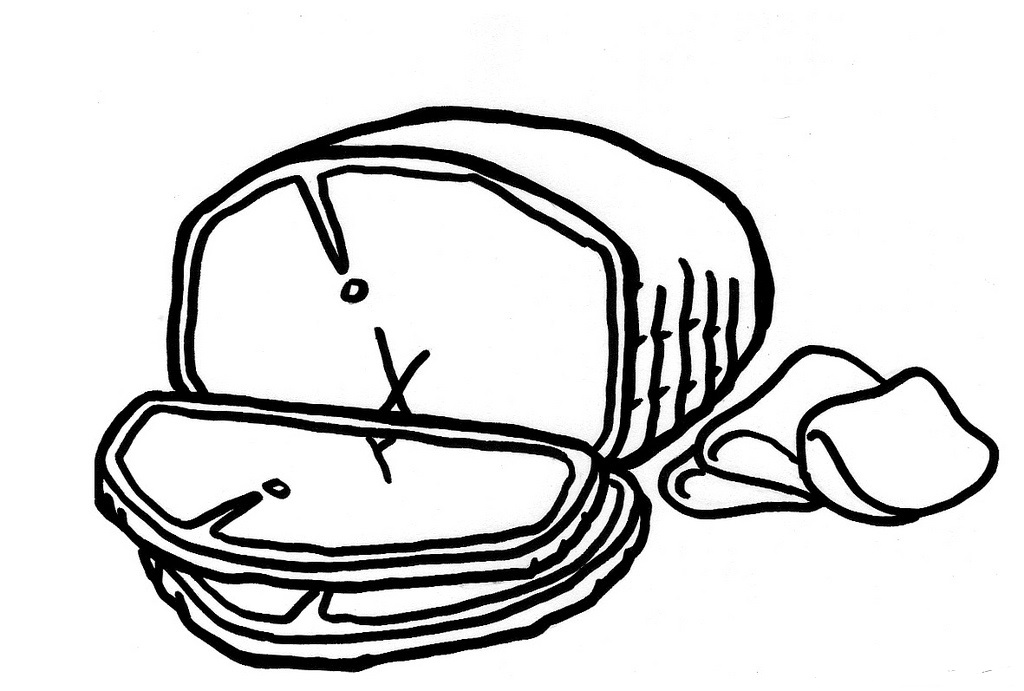
\includegraphics[width=0.4\textwidth]{ham}
\end{intersong}
\beginsong{Er is ham}
\beginverse
Er is ham, ham , voor op den boterham,
In de tent, in de tent, in de tent, in de tent,
Er is ham, ham, voor op den boterham,
In de fouragemeesters tent. 
\endverse
\beginchorus
Dat wist ik niet en bovendien, \rep{2}
Dat kon ik zonder bril niet zien   
\endchorus
\beginverse
Er is kaas, kaas, zo oud als sinterklaas.
\endverse
\beginverse
Er is soep, soep, voor een hongerige troep.
\endverse
\beginverse
Er is bier, bier, voor den aalmoezenier.
\endverse
\beginverse
Er is cake, cake, althans wat er op leek.
\endverse
\beginverse
Er is friet, friet, voor ieder een marmite. 
\endverse
\beginverse
Er is melk, melk, voor onze kleinste welp. 
\endverse
\beginverse
Er is cake, cake, vers van verleden week. 
\endverse
\endsong